\documentclass[12pt, titlepage]{article}

\usepackage{fullpage}
\usepackage[round]{natbib}
\usepackage{multirow}
\usepackage{booktabs}
\usepackage{tabularx}
\usepackage{graphicx}
\usepackage{float}
\usepackage{hyperref}
\hypersetup{
    colorlinks,
    citecolor=black,
    filecolor=black,
    linkcolor=red,
    urlcolor=blue
}

%% Comments

%\usepackage{color}
\usepackage[dvipsnames]{xcolor}

\newif\ifcomments\commentstrue

\ifcomments
\newcommand{\authornote}[3]{\textcolor{#1}{[#3 ---#2]}}
\newcommand{\todo}[1]{\textcolor{red}{[TODO: #1]}}
\else
\newcommand{\authornote}[3]{}
\newcommand{\todo}[1]{}
\fi

\newcommand{\wss}[1]{\authornote{blue}{SS}{#1}}
\newcommand{\an}[1]{\authornote{magenta}{Author}{#1}}
\newcommand{\meow}[1]{\authornote{Orchid}{JG}{#1}}


\newcounter{acnum}
\newcommand{\actheacnum}{AC\theacnum}
\newcommand{\acref}[1]{AC\ref{#1}}

\newcounter{ucnum}
\newcommand{\uctheucnum}{UC\theucnum}
\newcommand{\uref}[1]{UC\ref{#1}}

\newcounter{mnum}
\newcommand{\mthemnum}{M\themnum}
\newcommand{\mref}[1]{M\ref{#1}}

% jen stuff
\newcommand{\progname}{Kaplan} % PUT YOUR PROGRAM NAME HERE

\begin{document}

\title{Module Guide: \progname{} \wss{include software's name}} 
\author{Jen Garner}
\date{\today}

\maketitle

\pagenumbering{roman}

\section{Revision History}

\begin{tabularx}{\textwidth}{p{3cm}p{2cm}X}
\toprule {\bf Date} & {\bf Version} & {\bf Notes}\\
\midrule
November 5th, 2018 (Monday) & 1.0 & First draft \\
\bottomrule
\end{tabularx}

\newpage

\tableofcontents

\listoftables

\listoffigures

\newpage

\pagenumbering{arabic}

\section{Introduction}

Decomposing a system into modules is a commonly accepted approach to developing
software.  A module is a work assignment for a programmer or programming
team~\citep{ParnasEtAl1984}.  We advocate a decomposition
based on the principle of information hiding~\citep{Parnas1972a}.  This
principle supports design for change, because the ``secrets'' that each module
hides represent likely future changes.  Design for change is valuable in SC,
where modifications are frequent, especially during initial development as the
solution space is explored.  

Our design follows the rules layed out by \citet{ParnasEtAl1984}, as follows:
\begin{itemize}
\item System details that are likely to change independently should be the
  secrets of separate modules.
\item Each data structure is used in only one module.
\item Any other program that requires information stored in a module's data
  structures must obtain it by calling access programs belonging to that module.
\end{itemize}

After completing the first stage of the design, the Software Requirements
Specification (SRS), the Module Guide (MG) is developed~\citep{ParnasEtAl1984}. The MG
specifies the modular structure of the system and is intended to allow both
designers and maintainers to easily identify the parts of the software.  The
potential readers of this document are as follows:

\begin{itemize}
\item New project members: This document can be a guide for a new project member
  to easily understand the overall structure and quickly find the
  relevant modules they are searching for.
\item Maintainers: The hierarchical structure of the module guide improves the
  maintainers' understanding when they need to make changes to the system. It is
  important for a maintainer to update the relevant sections of the document
  after changes have been made.
\item Designers: Once the module guide has been written, it can be used to
  check for consistency, feasibility and flexibility. Designers can verify the
  system in various ways, such as consistency among modules, feasibility of the
  decomposition, and flexibility of the design.
\end{itemize}

The rest of the document is organized as follows. Section
\ref{SecChange} lists the anticipated and unlikely changes of the software
requirements. Section \ref{SecMH} summarizes the module decomposition that
was constructed according to the likely changes. Section \ref{SecConnection}
specifies the connections between the software requirements and the
modules. Section \ref{SecMD} gives a detailed description of the
modules. Section \ref{SecTM} includes two traceability matrices. One checks
the completeness of the design against the requirements provided in the SRS. The
other shows the relation between anticipated changes and the modules. Section
\ref{SecUse} describes the use relation between modules.

\section{Anticipated and Unlikely Changes} \label{SecChange}

This section lists possible changes to the system. According to the likeliness
of the change, the possible changes are classified into two
categories. Anticipated changes are listed in Section \ref{SecAchange}, and
unlikely changes are listed in Section \ref{SecUchange}.

\subsection{Anticipated Changes} \label{SecAchange}

Anticipated changes are the source of the information that is to be hidden
inside the modules. Ideally, changing one of the anticipated changes will only
require changing the one module that hides the associated decision. The approach
adapted here is called design for
change.

\begin{description}
\item[\refstepcounter{acnum} \actheacnum \label{acHardware}:] Hardware used to 
run the software.
\item[\refstepcounter{acnum} \actheacnum \label{acInput}:] Format of the input 
data.
\item[\refstepcounter{acnum} \actheacnum \label{acRMSD}:] RMSD module may be
  rewritten as a behaviour hiding module. \wss{A module doesn't really change
    its classification.  You can rewrite modules, but this isn't considered in
    this list of anticipated changes.  The anticipated changes imply that code
    will be re-written.  You might be getting confused because the software
    decision hiding modules are generic services that are often already
    available from other libraries.  However, even if you write the generic
    services yourself, it is still a software decision hiding module.}
\item[\refstepcounter{acnum} \actheacnum \label{acRing}:] The ring may change 
to another data structure. \wss{Can you create an abstract data structure that
  anticipates the future possibilities?}
\item[\refstepcounter{acnum} \actheacnum \label{acFit_G}:] The calculation for 
$Fit_G$ may be expanded to include more formats than initially described in the 
SRS document.
\item[\refstepcounter{acnum} \actheacnum \label{acHorton}:] \progname{} may be 
incorporated into another software package, thus making it a library not a 
standalone program. \wss{This isn't what is meant by anticipated changes.}
\item[\refstepcounter{acnum} \actheacnum \label{acOutputDevice}:] As per 
AC\ref{acHorton}, \progname{} may be required to run on cell phones through a 
web 
interface. The input/output device therefore will change from a keyboard and 
mouse to a touchscreen.
\item[\refstepcounter{acnum} \actheacnum \label{acProgLang}:] The programming 
language may change to improve performance. \wss{This isn't what is meant by anticipated changes.}
\item[\refstepcounter{acnum} \actheacnum \label{acEnergy}:] The external 
program used to run the energy calculations may change or multiple choices may 
become available (depending on user input).
\end{description}

\wss{There seems to be some misunderstanding about the anticipated changes.
  These are what become the secrets of your modules.  The interface to your
  modules will be abstract so that you can hide the anticipated changes in one
  module.  Changing programming language is not something you can ``hide'' in
  one module.  It would mean changing all of your modules.}

\subsection{Unlikely Changes} \label{SecUchange}

The module design should be as general as possible. However, a general system is
more complex. Sometimes this complexity is not necessary. Fixing some design
decisions at the system architecture stage can simplify the software design. If
these decision should later need to be changed, then many parts of the design
will potentially need to be modified. Hence, it is not intended that these
decisions will be changed.

\begin{description}
\item[\refstepcounter{ucnum} \uctheucnum \label{ucGA}:] The genetic algorithm 
component is unlikely to be exchanged for another algorithm.
\item[\refstepcounter{ucnum} \uctheucnum \label{ucEnery}:] The energy is 
unlikely to be calculated using methods other than those from quantum mechanics.
\item[\refstepcounter{ucnum} \uctheucnum \label{ucgoal}:] The goal of 
\progname{} is unlikely to change from locating conformers.
\end{description}

\section{Module Hierarchy} \label{SecMH}

This section provides an overview of the module design. Modules are summarized
in a hierarchy decomposed by secrets in Table \ref{TblMH}. The modules listed
below, which are leaves in the hierarchy tree, are the modules that will
actually be implemented.

\begin{description}
\item [\refstepcounter{mnum} \mthemnum \label{mHH}:] Hardware-Hiding
\item [\refstepcounter{mnum} \mthemnum \label{mGAIn}:] GA Input
\item [\refstepcounter{mnum} \mthemnum \label{mMolIn}:] Molecule Input
\item [\refstepcounter{mnum} \mthemnum \label{mGAC}:] GA Control
\item [\refstepcounter{mnum} \mthemnum \label{mFitg}:] $Fit_G$
\item [\refstepcounter{mnum} \mthemnum \label{mTour}:] Tournament
\item [\refstepcounter{mnum} \mthemnum \label{mCM}:] Crossover \& Mutation
\item [\refstepcounter{mnum} \mthemnum \label{mRing}:] Ring
\item [\refstepcounter{mnum} \mthemnum \label{mPmem}:] Pmem
\item [\refstepcounter{mnum} \mthemnum \label{mOut}:] Output
\item [\refstepcounter{mnum} \mthemnum \label{mGeometry}:] Geometry
\item [\refstepcounter{mnum} \mthemnum \label{mE}:] Energies
\item [\refstepcounter{mnum} \mthemnum \label{mRMSD}:] RMSD
\end{description}


\begin{table}[h!]
\centering
\begin{tabular}{p{0.3\textwidth} p{0.6\textwidth}}
\toprule
\textbf{Level 1} & \textbf{Level 2}\\
\midrule

{Hardware-Hiding Module} & ~ \\
\midrule

\multirow{9}{0.3\textwidth}{Behaviour-Hiding Module}& GA Input \\
													& Molecule Input \\
													& GA Control\\
													& $Fit_G$ \\
													& Tournament \\
													& Crossover \& Mutation \\
													& Ring \\
													& Pmem \\
													& Output \\

\midrule

\multirow{3}{0.3\textwidth}{Software Decision Module} & Geometry \\
													  & Energies \\
													  & RMSD \\
\bottomrule

\end{tabular}
\caption{Module Hierarchy}
\label{TblMH}
\end{table}

\section{Connection Between Requirements and Design} \label{SecConnection}

The design of the system is intended to satisfy the requirements developed in
the SRS. In this stage, the system is decomposed into modules. The connection
between requirements and modules is listed in Table \ref{TblRT}.

\section{Module Decomposition} \label{SecMD}

Modules are decomposed according to the principle of ``information hiding''
proposed by \citet{ParnasEtAl1984}. The \emph{Secrets} field in a module
decomposition is a brief statement of the design decision hidden by the
module. The \emph{Services} field specifies \emph{what} the module will do
without documenting \emph{how} to do it. For each module, a suggestion for the
implementing software is given under the \emph{Implemented By} title. If the
entry is \emph{OS}, this means that the module is provided by the operating
system or by standard programming language libraries.  Also indicate if the
module will be implemented specifically for the software.

Only the leaf modules in the
hierarchy have to be implemented. If a dash (\emph{--}) is shown, this means
that the module is not a leaf and will not have to be implemented. Whether or
not this module is implemented depends on the programming language
selected.

\subsection{Hardware Hiding Modules (\mref{mHH})}

\begin{description}
\item[Secrets:]The data structure and algorithm used to implement the virtual
  hardware.
\item[Services:]Serves as a virtual hardware used by the rest of the
  system. This module provides the interface between the hardware and the
  software. So, the system can use it to display outputs or to accept inputs.
\item[Implemented By:] OS
\end{description}

\subsection{Behaviour-Hiding Module}

\begin{description}
\item[Secrets:]The contents of the required behaviours.
\item[Services:]Includes programs that provide externally visible behaviour of
  the system as specified in the software requirements specification (SRS)
  documents. This module serves as a communication layer between the
  hardware-hiding module and the software decision module. The programs in this
  module will need to change if there are changes in the SRS.
\item[Implemented By:] --
\end{description}

\subsubsection{GA Input Module (\mref{mGAIn})}

\begin{description}
\item[Secrets:]The format and structure of the input data for the genetic 
algorithm, including how the input data is verified.
\item[Services:] Communicates the size of the Ring data structure, the number 
of mating events to perform, the maximum number of mutations, the maximum 
number of swaps, the number of conformers in the optimization, the size of the 
initial population, and which fitness function to use to \mref{mGAC}. Ensures 
all input data is of the correct type and within reasonable 
bounds. These values are static and should not change during the optimization.
\item[Implemented By:] \progname{}
\end{description}

\subsubsection{Molecule Input Module (\mref{mMolIn})}
\begin{description}
	\item[Secrets:] The format and structure of the input data for the 
	molecule, including how the input data is verified.
	\item[Services:] Reads in a molecular structure data file input and 
	verifies the types, values, and completeness of the input.
	\item[Implemented By:] \progname{}
\end{description}

\subsubsection{GA Control Module (\mref{mGAC})}

\begin{description}
	\item[Secrets:] How the pieces of the genetic algorithm work together to 
	find and optimize conformer geometries.
	\item[Services:] Initializes the Ring data structure and calls the 
	Tournament to update the Ring. When the number of mating events specified 
	by the user has been completed, calls the Output module. 
	\item[Implemented By:] \progname{}
\end{description}

\subsubsection{$Fit_G$ Module (\mref{mFitg})}

\begin{description}
	\item[Secrets:] How to calculate the fitness of a set of conformers.
	\item[Services:] Calculate the fitness of given population members from the 
	Ring.
	\item[Implemented By:] \progname{}
\end{description}

\subsubsection{Tournament Module (\mref{mTour})}

\begin{description}
	\item[Secrets:] How to compare the set of available solutions (in the Ring 
	\mref{mRing}) for the conformer optimization problem.
	\item[Services:] Chooses participants and winners in the 
	tournament. Returns children (made by \mref{mCM}) such that these 
	population members can be given to the Ring.
	\item[Implemented By:] \progname{}
\end{description}

\subsubsection{Crossover \& Mutation Module (\mref{mCM})}

\begin{description}
	\item[Secrets:] How to generate new population members.
	\item[Services:] Generates new population members to put in the Ring data 
	structure.
	\item[Implemented By:] \progname{}
\end{description}

\subsubsection{Ring Module (\mref{mRing})}

\begin{description}
	\item[Secrets:] The data structure for the Ring (the population of 
	solutions).
	\item[Services:] Determines if a new population member (Pmem) can be added, 
	and where they are added.
	\item[Implemented By:] \progname{}
\end{description}


\subsubsection{Pmem Module (\mref{mPmem})}

\begin{description}
	\item[Secrets:] The data structure for the individual solutions to the 
	conformer search optimization problem.
	\item[Services:] Defines the potential solutions to the conformer 
	optimization in the form of dihedral angles (and energies if calculated). 
	\item[Implemented By:] \progname{}
\end{description}

\subsubsection{Output Module (\mref{mOut})}

\begin{description}
	\item[Secrets:] The format and content of the output data.
	\item[Services:] Provides the results of the conformer optimization to the 
	user. Receives the input geometry from \mref{mGAC} to reconstruct the new 
	conformer geometries. 
	\item[Implemented By:] \progname{}
\end{description}

\subsection{Software Decision Module}

\begin{description}
\item[Secrets:] The design decision based on mathematical theorems, physical
  facts, or programming considerations. The secrets of this module are
  \emph{not} described in the SRS.
\item[Services:] Includes data structure and algorithms used in the system that
  do not provide direct interaction with the user. 
  % Changes in these modules are more likely to be motivated by a desire to
  % improve performance than by externally imposed changes.
\item[Implemented By:] --
\end{description}

\subsubsection{Geometry Module (\mref{mGeometry})}
\begin{description}
	\item[Secrets:] Data structure for full geometric specifications.
	\item[Services:] Combines a list of dihedral angles and the original 
	molecular geometry to produce a new geometry. Creates an object capable of 
	reading and writing structure files.
	\item[Implemented By:] Vetee, Openbabel \citet{obabel} \citet{obabel-web}
\end{description}

\subsubsection{Energies Module (\mref{mE})}
\begin{description}
	\item[Secrets:] How to calculate the energy of a conformer geometry.
	\item[Services:] Calculates the energy for a given geometry based on 
	user-specified basis set and method. 
	\item[Implemented By:] Psi4 \citet{psi4}, Gaussian \citet{g16}, 
	Horton \citet{horton}
\end{description}

\subsubsection{RMSD Module (\mref{mRMSD})}
\begin{description}
	\item[Secrets:] How to calculate the root-mean-square deviation for a set 
	of conformers.
	\item[Services:] Calculates the RMSD for a set of geometries.
	\item[Implemented By:] rmsd\citet{rmsd-charnley}
\end{description}


\section{Traceability Matrix} \label{SecTM}

This section shows two traceability matrices: between the modules and the
requirements and between the modules and the anticipated changes.

% the table should use mref, the requirements should be named, use something
% like fref
\begin{table}[H]
\centering
\begin{tabular}{p{0.2\textwidth} p{0.6\textwidth}}
\toprule
\textbf{Req.} & \textbf{Modules}\\
\midrule
R1 & \mref{mMolIn} \\
R2 & \mref{mFitg}, \mref{mRing} \\
R3 & \mref{mFitg}, \mref{mRMSD}, \mref{mE} \\
R4 & \mref{mFitg}, \mref{mE} \\
R5 & \mref{mOut}, \mref{mMolIn} \\
NFR1 & \mref{mFitg} \\
NFR2 & M2-M11, but especially \mref{mGAC} \\
NFR3 & M2-M11 \\
NFR4 & \mref{mMolIn}, \mref{mGAIn} \\
NFR5 & \mref{mE}, \mref{mRMSD}, \mref{mMolIn}, \mref{mOut} \\
\bottomrule
\end{tabular}
\caption{Trace between requirements and modules.}
\label{TblRT}
\end{table}

As in Table \ref{trace-ACM}, there are two modules that change as a result of 
\acref{acInput}. The input will be divided into two modules - one module 
(\mref{mGAIn}) is responsible for handling the genetic algorithm inputs and the 
other module (\mref{mMolIn}) is responsible for handling the molecular inputs. 
The author has already written a software package that can handle molecular 
geometry (and its conversion to other formats). This package also interfaces 
with Openbabel \cite{obabel}. The author has decided to use a Behaviour-Hiding 
module for the genetic algorithm, as these algorithms are very dependent on the 
format of the data structure used to represent the problem (and thus converting 
to a format acceptable to another external program might change the results 
significantly). Furthermore, one of the goals of the program is to make the 
package work on high-performance computing clusters. If there are fewer 
external programs necessary to run \progname{}, then it will be easier to 
install the program. All modules will change upon change of the programming 
language, hence the reason \acref{acProgLang} is linked to all Behaviour-Hiding 
and Software Decision modules.

\begin{table}[H]
\centering
\begin{tabular}{p{0.2\textwidth} p{0.6\textwidth}}
\toprule
\textbf{AC} & \textbf{Modules}\\
\midrule
\acref{acHardware} & \mref{mHH}\\
\acref{acInput} & \mref{mMolIn} \mref{mGAIn} \\
\acref{acRMSD} & \mref{mRMSD} \\
\acref{acRing} & \mref{mRing} \\
\acref{acFit_G} & \mref{mFitg} \\
\acref{acHorton} & \mref{mGAC} \\
\acref{acOutputDevice} & \mref{mOut} \\
\acref{acProgLang} & M2-M11 \\
\acref{acEnergy} & \mref{mE} \\
\bottomrule
\end{tabular}
\caption{Trace between anticipated changes and modules.}
\label{trace-ACM}
\end{table}

\section{Use Hierarchy Between Modules} \label{SecUse}

In this section, the uses hierarchy between modules is
provided. \citet{Parnas1978} said of two programs A and B that A {\em uses} B if
correct execution of B may be necessary for A to complete the task described in
its specification. That is, A {\em uses} B if there exist situations in which
the correct functioning of A depends upon the availability of a correct
implementation of B.  Figure \ref{FigUH} illustrates the use relation between
the modules. It can be seen that the graph is a directed acyclic graph
(DAG). Each level of the hierarchy offers a testable and usable subset of the
system, and modules in the higher level of the hierarchy are essentially simpler
because they use modules from the lower levels.

\begin{figure}[H]
\centering
%\includegraphics[width=0.7\textwidth]{UsesHierarchy.png}
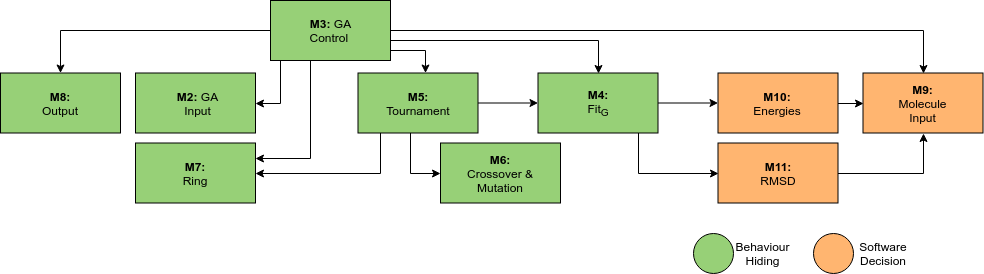
\includegraphics[width=\textwidth]{MG_hierarchy_draft4.png}
\caption{Use hierarchy among modules. Note the hardware-hiding module has been 
omitted for clarity.}
\label{FigUH}
\end{figure}

\wss{Do any other modules use the Input module?  It is usually the case that
  other modules will ask the Input module for its values.  Or will the Control
  module be the only one that needs these values?}

%\section*{References}

\bibliographystyle {plainnat}
\bibliography{../../../ReferenceMaterial/References}

\end{document}